\documentclass[11pt]{article}

\usepackage[margin=1in]{geometry}
\usepackage[T1]{fontenc}
\usepackage{lmodern}
\usepackage{microtype}
\usepackage{amsmath,amssymb,amsthm, mathtools}
\usepackage[dvipsnames]{xcolor}
\usepackage{enumitem}
\usepackage{hyperref}
\usepackage{graphicx}
\usepackage{xcolor}
\usepackage{xypic}
\usepackage[all,line,color]{xy}
\usepackage{graphicx}
\usepackage{pagecolor}
\pagecolor{white}
\usepackage{hyperref}
\usepackage{wrapfig
}\usepackage{caption}
\usepackage{tikz}
\usetikzlibrary{arrows.meta}
\usepackage{amsmath,amssymb}
\usepackage{algorithm}
\usepackage{algpseudocode}

\captionsetup[figure]{
  format=plain,
  justification=justified,
  singlelinecheck=false,
  margin=1.75cm,
  font=small
}

\hypersetup{
  colorlinks=true,
  linkcolor=MidnightBlue,
  citecolor=MidnightBlue,
  urlcolor=MidnightBlue
}

\setlength{\parindent}{0pt}
\setlength{\parskip}{0.75em}

\newcommand{\SC}{\texttt{state\_collapser}}
\newcommand{\logHRL}{\texttt{logHRL}}
\newcommand{\trop}{\mathrm{trop}}
\newcommand{\A}{\mathcal A}
\newcommand{\Sset}{\mathcal S}
\newcommand{\R}{\mathbb R}

\newenvironment{claimbox}
  {\begin{quote}\itshape}
  {\end{quote}}

\newenvironment{dictionary}
  {\begin{quote}\begin{tabular}{@{}p{0.30\linewidth}c p{0.54\linewidth}@{}}}
  {\end{tabular}\end{quote}}

\title{Log/Tropical Geometry and the Quotient-Tower Picture}
\author{Research-design note for \SC}
\date{May 2026}

\begin{document}

\maketitle

\section*{Status}

This is a research-design note, not a settled theorem.

It records a mathematical discussion about whether the \logHRL{}
quotient-tower construction should be understood not merely as being analogous
to tropical geometry, but as a finite, algorithmic reconfiguration of the same
logarithmic operation that appears in first-wave tropical geometry.

\section*{Attribution}

The central conceptual claim in this note is due to the Project Owner.

The Project Owner introduced the stronger thesis that the TeX research document
is not merely borrowing tropical language, but may be reconfiguring the entire
log/tropical geometry picture in the setting of reinforcement-learning
state/action path geometry. The Project Owner also directed the discussion away
from later adic/valuation analytic geometry and toward the first-wave
coordinatewise logarithmic construction of amoebas and tropical limits.

The core Project Owner question was:

\begin{claimbox}
Can the logarithm that appears in the path-volume/log-speed-up theorem be the
same logarithm that appears in tropical geometry, with the logarithm observed in
a different part of the construction?
\end{claimbox}

The assistant contribution here is organizational: making the dictionary
explicit, identifying semiring dequantization as the cleanest bridge, separating
strong points from weak points, and writing down theorem-shaped formulations
that could guide future mathematical work.

\section{Starting Claim}

The strong claim under discussion is:

\begin{claimbox}
The quotient-tower construction in \logHRL{} is not just loosely reminiscent of
tropical geometry. It may be a finite, algorithmic version of the same
logarithmic simplification that produces tropical geometry.
\end{claimbox}

The guiding phrase that emerged in the discussion is:

\begin{claimbox}
loss of fine coordinates while preserving asymptotic decision geometry.
\end{claimbox}

This is the point of contact. Tropical geometry discards fine coordinate data
while preserving dominance, order-of-growth, and combinatorial incidence data
relevant to the computation. The quotient tower discards fine state/action
identity while preserving the outgoing decision geometry relevant to
hierarchical control.

\section{First-Wave Tropicalization}

The relevant tropical picture is the early coordinatewise logarithmic one. One
starts with a point in a positive or complex torus and applies a logarithmic
map:

\[
(z_1,\dots,z_n)
\longmapsto
(\log_b |z_1|,\dots,\log_b |z_n|).
\]

For a fixed coordinate value, changing the base alone is only a rescaling:

\[
\log_b x
=
\frac{\log x}{\log b}.
\]

So the base change is not interesting by itself. It becomes geometrically
meaningful when applied to a family whose coordinates scale with the base:

\[
x_b \sim c b^\alpha.
\]

Then

\[
\log_b x_b \to \alpha.
\]

The logarithm has discarded the coefficient \(c\) and retained the exponent,
order-of-growth, or dominance datum \(\alpha\).

This is the relevant mathematical action:

\begin{claimbox}
exact coordinate values are forgotten; scale/dominance data are retained.
\end{claimbox}

\section{The Amoeba as the Tier-Zero Analogue}

One way to place the quotient tower next to this picture is:

\begin{claimbox}
apply one logarithmic map and obtain an amoeba; pretend this amoeba is the
analogue of \(G_t^0\).
\end{claimbox}

This is not because the amoeba is literally a graph. The point is that the
amoeba is still close to the original variety: it is a transformed image that
has not yet collapsed all the way to a tropical skeleton.

In the state/action setting, \(G_t^0\) plays a similar role. It is already a
discovered, combinatorial representation of the environment, but it is still
the finest available tier. It has not yet been coarsened into the quotient
tower.

The possible analogy is:

\begin{dictionary}
amoeba after one log map
  & \(\longleftrightarrow\) &
discovered base graph \(G_t^0\) \\
tropical limiting skeleton
  & \(\longleftrightarrow\) &
coarser tiers \(G_t^i\) \\
full scale-dependent contraction process
  & \(\longleftrightarrow\) &
quotient tower \(G_t^0\to G_t^1\to\cdots\to G_t^N\)
\end{dictionary}

\section{How the Tier Index \texorpdfstring{\(i\)}{i} Is Like the Logarithmic Base \texorpdfstring{\(b\)}{b}}

The tier index \(i\) is not literally the base \(b\).

The better formulation is:

\begin{claimbox}
\(i\) is a discrete event index along a logarithmic visibility flow.
\end{claimbox}

If one changes \(b\) in a raw logarithmic map, then for two fixed positive
numbers \(x,y\),

\[
\log_b x-\log_b y
=
\frac{\log x-\log y}{\log b}.
\]

As \(b\) increases, their distance in log-coordinates shrinks. With infinite
precision this is only rescaling. But with a fixed observational threshold,
decision resolution, or dominance criterion, more distinctions become invisible
as \(b\) varies.

Thus, a meaningful dictionary is:

\begin{dictionary}
base \(b\)
  & \(\longrightarrow\) &
continuous logarithmic resolution parameter \\
tier \(i\)
  & \(\longrightarrow\) &
discrete quotient event along that resolution parameter \\
\(G_t^i\)
  & \(\longrightarrow\) &
graph/decision geometry after distinctions invisible at scale \(b_i\)
have been contracted \\
\(\Sigma_0^i\)
  & \(\longrightarrow\) &
edge list whose distinctions die between scale \(b_{i-1}\) and \(b_i\)
\end{dictionary}

Equivalently, set

\[
\varepsilon
=
\frac{1}{\log b}.
\]

Then increasing \(b\) decreases \(\varepsilon\), so increasingly fine subscale
distinctions disappear. The quotient tower records the finitely many critical
moments at which this loss of visibility changes the combinatorial decision
structure.

This is the honest version:

\begin{claimbox}
The tower is not the raw family of maps \(\log_b\); it is the event-quotient of
that family after imposing a finite decision-resolution relation.
\end{claimbox}

\section{The Same Logarithm: Semiring Dequantization}

The cleanest way to make the phrase ``the same logarithm'' precise is semiring
dequantization.

Consider

\[
\operatorname{Log}_b(x):=\log_b x.
\]

This sends multiplication to addition exactly:

\[
\log_b(xy)=\log_b x+\log_b y.
\]

It sends addition to log-sum-exp:

\[
\log_b(x+y)
=
\log_b\left(b^{\log_b x}+b^{\log_b y}\right).
\]

In the limit,

\[
\log_b\left(b^{a_1}+\cdots+b^{a_n}\right)
\longrightarrow
\max_i a_i
\qquad
(b\to\infty).
\]

Thus the logarithm deforms the positive semiring into the max-plus semiring:

\begin{dictionary}
ordinary addition
  & \(\longrightarrow\) &
log-sum-exp \(\longrightarrow\) max \\
ordinary multiplication
  & \(\longrightarrow\) &
addition
\end{dictionary}

This is the same algebraic move in tropical geometry and in Bellman-style
optimal control.

\section{Tropical Geometry Side}

For a polynomial
\[
f(z)
=
\sum_m c_m z^m,
\]
set
\[
z_j=b^{x_j}.
\]
Then the monomial \(c_m z^m\) becomes
\[
c_m z^m
=
c_m b^{\langle m,x\rangle}.
\]
After taking logarithms:
\[
\log_b |c_m z^m|
=
\log_b |c_m|+\langle m,x\rangle.
\]

The full sum is governed, in the tropical limit, by the dominant term:

\[
\log_b
\left|
\sum_m c_m b^{\langle m,x\rangle}
\right|
\rightsquigarrow
\max_m
\left\{
\log_b |c_m|+\langle m,x\rangle
\right\}.
\]

So algebraic addition of monomials becomes tropical maximum over dominant
monomials. The hard algebro-geometric object is replaced by a polyhedral
dominance object.

This is why tropical geometry can accelerate or simplify computations such as
intersection-theoretic computations: the logarithm moves the problem from fine
coordinate geometry to combinatorial dominance geometry.

\section{RL / Path Geometry Side}

In reinforcement learning or path geometry, the analogous ``terms'' are not
monomials but paths.

Let a trajectory \(\gamma\) have reward, negative cost, or energy
\(R(\gamma)\), and define a positive path weight

\[
W_b(\gamma)
=
b^{R(\gamma)}.
\]

The path partition function from a state \(s\) is

\[
Z_b(s)
=
\sum_{\gamma:s\leadsto *} b^{R(\gamma)}.
\]

Applying the same logarithm gives

\[
\log_b Z_b(s)
=
\log_b
\left(
\sum_{\gamma:s\leadsto *} b^{R(\gamma)}
\right)
\longrightarrow
\max_{\gamma:s\leadsto *} R(\gamma).
\]

This is the Bellman/tropical operation. The ordinary sum over possible paths
degenerates to the optimal path. The same logarithm that tropicalizes sums of
monomials also tropicalizes sums over trajectories.

The dictionary is:

\begin{dictionary}
tropical geometry
  & \(\longrightarrow\) &
sum over monomials; \(\log_b\); dominant monomial survives \\
RL/path geometry
  & \(\longrightarrow\) &
sum over paths/actions; \(\log_b\); optimal path/action survives
\end{dictionary}

This is a concrete sense in which the logarithm is the same logarithm.

\section{Direct Image Along Quotients}

The direct-image discussion is especially important because it explains why max
aggregation is not merely an engineering choice.

Let

\[
q:S\to \bar S
\]

be a quotient map. An ordinary pushforward over a fiber might be

\[
(q_*F)(\bar s)
=
\sum_{s\in q^{-1}(\bar s)} F(s).
\]

If

\[
F(s)=b^{V(s)},
\]

then

\[
\log_b
\left(
\sum_{s\in q^{-1}(\bar s)} b^{V(s)}
\right)
\longrightarrow
\max_{s\in q^{-1}(\bar s)} V(s).
\]

So the tropical direct image is

\[
(q_*^{\mathrm{trop}}V)(\bar s)
=
\max_{s\in q^{-1}(\bar s)} V(s).
\]

This matches the PO observation that, for many RL problems, a max direct image
is more natural than an average direct image because the coarser state should
remember the best available downstream value, not the average value of the
fiber.

In this language:

\begin{dictionary}
sum aggregation
  & \(\longrightarrow\) &
ordinary direct image \\
average aggregation
  & \(\longrightarrow\) &
normalized/probabilistic direct image \\
max aggregation
  & \(\longrightarrow\) &
tropical direct image \\
log-sum-exp / \(p\)-norm families
  & \(\longrightarrow\) &
dequantizing bridges between these regimes
\end{dictionary}

\section{Where the Log Is Observed}

The logarithm is visible in different places in the two stories.

In tropical geometry:

\begin{claimbox}
\(\log\) first, compute afterward.
\end{claimbox}

The logarithm is an explicit coordinate transformation:

\[
(z_1,\dots,z_n)
\mapsto
(\log_b |z_1|,\dots,\log_b |z_n|).
\]

In the quotient-tower RL story:

\begin{claimbox}
construct the tower, then observe logarithmic search/address complexity.
\end{claimbox}

The logarithm appears in the complexity theorem and in the Bellman/direct-image
algebra. The PO's stronger thesis is that this difference in where the
logarithm is observed may not be fundamental. The tower construction itself may
be the hidden logarithmic coordinate transformation for path-space geometry.

That is:

\begin{claimbox}
the quotient tower may be the log/tropicalization map for RL path geometry.
\end{claimbox}

The log-speed-up would then be the computational shadow of having passed from
flat path space to a tropical/combinatorial decision skeleton.

\section{Strong Formulation}

The strongest formulation currently on the table is:

\begin{claimbox}
The quotient tower is a finite, algorithmic log-limit of the state/action path
geometry.
\end{claimbox}

Equivalently:

\begin{claimbox}
Hierarchical quotient construction is tropicalization before passage to a
continuum limit.
\end{claimbox}

Or, in theorem-shaped language:

\begin{quote}
\itshape
Given a finite state/action graph with a compatible quotient tower and
semiring-valued reward or value data, the dequantized Bellman/direct-image
operators along the tower are max-plus pushforwards on the quotient skeletons.
If the ordered edge partition is induced by a logarithmic scale or dominance
filtration, then the quotient tower is the finite combinatorial skeleton of the
associated path-space tropicalization.
\end{quote}

This is not yet a theorem. It indicates the structure one would need to define
in order to make the statement theorem-grade.

\section{What Must Be Added To Make This More Than Analogy}

The weak point is that the current quotient tower can be built from an
arbitrary ordered edge partition:

\[
\A_t^0
=
\Sigma_0^1 \sqcup \cdots \sqcup \Sigma_0^d.
\]

An arbitrary ordered partition is not automatically a logarithmic scale
filtration.

To make the tropical/log identification honest, one needs extra structure, such
as:

\begin{itemize}[leftmargin=2em]
\item an edge/action distinguishability scale;
\item a reward/value dominance scale;
\item a path-volume contribution scale;
\item a decision-resolution threshold;
\item a valuation-like filtration on actions or path families;
\item a semiring-valued path partition function whose dequantization induces
the partition.
\end{itemize}

For example, one could seek a scale function

\[
\lambda:\A_t^0\to \R
\]

such that

\[
e\in \Sigma_0^i
\quad\Longleftrightarrow\quad
\lambda(e)\in [\lambda_i,\lambda_{i+1}).
\]

Then \(i\) becomes a discrete critical value of the logarithmic filtration, and
the tier construction is much closer to a literal tropicalization process.

Another possible route is to define an indistinguishability relation depending
on a logarithmic resolution parameter:

\[
s\sim_\varepsilon s'
\quad\Longleftrightarrow\quad
\text{the outgoing decision data of }s,s'
\text{ differ only below resolution }\varepsilon.
\]

Then the tower could be recovered at critical values

\[
\varepsilon_i=\frac{1}{\log b_i}.
\]

This would make precise the slogan:

\begin{claimbox}
\(i\) is a discrete scale index for the log-base flow.
\end{claimbox}

\section{Possible Commutative Diagram}

A future theorem might be organized around a diagram of this form:

\[
\begin{array}{ccc}
\text{positive path weights on }G_t^0
& \xrightarrow{\quad q_*\quad} &
\text{positive fiber/path aggregates on }G_t^i
\\[0.4em]
\downarrow \log_b
&&
\downarrow \log_b
\\[0.4em]
\text{dequantized values on }G_t^0
& \xrightarrow{\quad q_*^{\mathrm{trop}}\quad} &
\text{max-plus fiber/path values on }G_t^i
\end{array}
\]

In the limit \(b\to\infty\), the bottom horizontal map should be the tropical
direct image:

\[
(q_*^{\mathrm{trop}}V)(\bar s)
=
\max_{s\in q^{-1}(\bar s)}V(s).
\]

The question is whether the quotient tower itself can also be recovered from
the same dequantizing scale data, rather than merely being a useful structure
on which the dequantized operators act.

\section{Strong Points Of The Analogy}

The touch points that currently look mathematically serious are:

\begin{itemize}[leftmargin=2em]
\item Both stories replace fine coordinate geometry by scale/dominance
geometry.
\item Both stories turn sums into maxima through the same logarithmic limiting
operation.
\item Both stories produce combinatorial skeletons that preserve the data
relevant to the computation.
\item Both stories simplify hard computations by moving from flat/fine geometry
to structured quotient or polyhedral geometry.
\item The RL Bellman operator is naturally max-plus, which is precisely the
tropical semiring.
\item Max direct image along quotient fibers is exactly the tropicalization of
sum direct image.
\item The tier index \(i\) can plausibly be interpreted as a discrete critical
index along a logarithmic scale filtration.
\end{itemize}

\section{Weak Points Of The Analogy}

The main weak points are:

\begin{itemize}[leftmargin=2em]
\item Changing \(b\) alone only rescales a fixed logarithmic image.
\item A quotient tower built from an arbitrary edge partition is not
automatically a tropical object.
\item Tropical geometry usually begins with algebraic equations, monomials, and
coordinates; the RL tower begins with a discovered transition graph and
contraction policy.
\item The current package architecture does not yet define the scale/valuation
structure that would force the ordered edge partition to be logarithmic.
\item The tower currently encodes decision equivalence, not necessarily
order-of-magnitude equivalence, unless those are identified by an additional
theorem or construction.
\end{itemize}

These weak points do not defeat the claim. They specify what has to be built or
proved.

\section{Research Tasks Suggested By This Discussion}

The immediate mathematical tasks are:

\begin{enumerate}[leftmargin=2em]
\item Define a scale or dominance filtration on state/action graphs that can
generate the ordered edge partition used by the tower.
\item Define path partition functions \(Z_b(s)\) and quotient fiber partition
functions compatible with tower morphisms.
\item Prove that \(\log_b\) dequantization turns ordinary path/fiber
aggregation into max-plus Bellman and direct-image aggregation.
\item Determine whether the tower partitions can be recovered as critical
equivalence classes of a logarithmic visibility relation.
\item Clarify when the quotient tower is a tropical skeleton of path geometry
rather than merely a useful hierarchical abstraction.
\item Identify the exact hypotheses under which the log-speed-up theorem and
tropical dequantization theorem become the same statement viewed from different
sides.
\end{enumerate}

\section{Provisional Bottom Line}

The conservative statement is:

\begin{claimbox}
The same logarithmic semiring dequantization that underlies first-wave tropical
geometry also underlies max-plus Bellman aggregation and max direct images along
quotient fibers.
\end{claimbox}

The stronger Project Owner thesis is:

\begin{claimbox}
The state/action quotient tower is itself the finite algorithmic analogue of
the tropical/logarithmic limiting process, with the tier index recording
discrete critical events in a logarithmic visibility flow.
\end{claimbox}

That stronger thesis is not established here, but it is now framed in a way
that looks mathematically attackable rather than merely metaphorical.

\section{Relation To Semiring-Valued Polynomial-Span Dataflow}

The Project Owner's reading is that the relevant Dudzik--Velickovic line of
work is structurally tropical, even when it is not advertised in those words.
That is: Dudzik is, in this sense, secretly operating as a tropical geometer.

This should not be stated as a claim about the authors' intent. The point is
structural. Dudzik--Velickovic foreground graph neural networks, dynamic
programming, polynomial spans, pullback, pushforward, bag/list monads,
semirings, and algorithmic alignment. But the tropical geometry is already
sitting inside the semiring choices.

The same point applies to the Gavranovic--Lessard--Dudzik--von Glehn--Araujo--
Velickovic categorical deep learning paper: the paper presents an algebraic
architecture story, but the moment the architecture is evaluated over tropical
or idempotent semirings, it is also a tropical-geometric story in disguise.

Their basic graph-dataflow template has the form

\[
[W,R]
\xrightarrow{i^*}
[X,R]
\xrightarrow{p_\otimes}
[Y,R]
\xrightarrow{o_\oplus}
[Z,R].
\]

Here \(R\) is the value or latent space, and the two aggregation operations
\(\otimes\) and \(\oplus\) supply the algebra needed to combine message
arguments and aggregate incoming messages. Their key observation is that the
same polynomial-span/integral-transform skeleton can describe both ordinary
GNN message passing and dynamic programming, once one chooses the appropriate
coefficient algebra.

On the dynamic-programming side, one naturally meets tropical semirings such as

\[
(\mathbb N\cup\{\infty\},\min,+)
\]

or sign-reversed max-plus variants. This is not an incidental coefficient
choice. It is the Bellman/tropical algebra of optimal path computation.

The present note adds the following extra interpretation. Dudzik--Velickovic
fix the graph/dataflow diagram, vary the semiring or latent value algebra, and
observe that GNNs and dynamic programming share the same abstract
polynomial-span computation. The present quotient-tower perspective treats the
passage between ordinary positive aggregation and tropical Bellman aggregation
as a logarithmic degeneration, views max-plus direct image as the
tropicalization of sum direct image, and asks whether the quotient tower itself
is the finite tropical skeleton of state/action path geometry.

So the connection is not merely that both stories mention semirings. The shared
structure is:

\[
\text{pullback}
\quad+\quad
\text{product-like local combination}
\quad+\quad
\text{sum/max-like pushforward aggregation}.
\]

In Dudzik--Velickovic, this appears as polynomial-span dataflow. In the
log/tropical quotient-tower picture, the same architecture is read through the
dequantizing map

\[
\log_b
\left(
\sum_i b^{a_i}
\right)
\longrightarrow
\max_i a_i.
\]

Thus a sum-type pushforward over a fiber,

\[
(q_*F_b)(\bar s)
=
\sum_{s\in q^{-1}(\bar s)} b^{V(s)},
\]

dequantizes to the tropical direct image

\[
(q_*^{\mathrm{trop}}V)(\bar s)
=
\max_{s\in q^{-1}(\bar s)}V(s).
\]

This is exactly the state/action quotient analogue of the message pushforward
\(o_\oplus\), with \(\oplus\) specialized to a tropical aggregator.

The rhetorical point should be made carefully:

\begin{claimbox}
Dudzik--Velickovic identify the semiring-polynomial-span form of graph message
passing and dynamic programming. The present perspective reads the tropical
semiring appearing in their dynamic-programming examples not as an isolated
coefficient choice, but as the logarithmic degeneration of ordinary positive
aggregation. This moves the semiring parameter itself into the geometry.
\end{claimbox}

The additional \SC{} contribution is the tower:

\[
G_t^0
\twoheadrightarrow
G_t^1
\twoheadrightarrow
\cdots
\twoheadrightarrow
G_t^N.
\]

The question is no longer only how to run semiring-valued dataflow on one
graph. The question is how semiring-valued dataflow behaves under quotient
maps, direct images, lifts, frozen tiers, and scale-indexed contraction events.
This is where the Project Owner's stronger log/tropical thesis genuinely goes
beyond the Dudzik--Velickovic setup.

\section{Literature Trail For This Connection}

The immediate machine-learning/categorical-dataflow literature is:

\begin{itemize}[leftmargin=2em]
\item \href{https://arxiv.org/abs/2203.15544}{Dudzik and Velickovic,
\textit{Graph Neural Networks are Dynamic Programmers}}. This is the closest
source. It identifies a polynomial-span/integral-transform skeleton common to
GNN message passing and dynamic programming, with semiring structure on the
latent/value space \(R\). The OpenReview page is
\href{https://openreview.net/forum?id=wu1Za9dY1GY}{here}.
\item \href{https://proceedings.mlr.press/v235/gavranovic24a.html}
{Gavranovic, Lessard, Dudzik, von Glehn, Araujo, and Velickovic,
\textit{Position: Categorical Deep Learning is an Algebraic Theory of All
Architectures}}. This places the Dudzik-style algebraic architecture
perspective inside a broader categorical deep learning program. The arXiv page
is \href{https://arxiv.org/abs/2402.15332}{here}, and the project page is
\href{https://categoricaldeeplearning.com/}{here}.
\item \href{https://arxiv.org/abs/1707.09227}{Dudzik,
\textit{Quantales and Hyperstructures: Monads, Mo' Problems}}. This is useful
background for why the semiring/quantale/hyperstructure thread in Dudzik's work
is not accidental.
\end{itemize}

The older dynamic-programming and path-problem background is:

\begin{itemize}[leftmargin=2em]
\item \href{https://www.cambridge.org/core/journals/mathematical-structures-in-computer-science/article/categories-relations-and-dynamic-programming/552525CAD62B986E5C7461DB55B3B952}
{de Moor, \textit{Categories, Relations and Dynamic Programming}}. This is one
of the categorical dynamic-programming sources explicitly used by
Dudzik--Velickovic.
\item \href{https://www.sciencedirect.com/science/article/pii/0012365X7990061X}
{Carre, \textit{Semirings and path spaces}}. This is a classical algebraic
path-problem source: graph path problems are treated through semiring-like
algebraic structure.
\item \href{https://link.springer.com/book/10.1007/978-3-031-79983-9}
{Baras and Theodorakopoulos, \textit{Path Problems in Networks}}. This is a
book-length treatment of the algebraic path problem and its applications.
\item \href{https://arxiv.org/abs/2005.06682}{Master, \textit{The Open
Algebraic Path Problem}}. This extends algebraic path problems to open networks
and emphasizes functoriality.
\item \href{https://graphblas.org/}{GraphBLAS}. This is the
engineering-standard version of the same semiring insight: graph algorithms can
be expressed as linear-algebraic operations over chosen semirings.
\end{itemize}

The polynomial-span/polynomial-functor background is:

\begin{itemize}[leftmargin=2em]
\item \href{https://arxiv.org/abs/0906.4931}{Gambino and Kock,
\textit{Polynomial functors and polynomial monads}}. This is a foundational
source for polynomial functors and polynomial monads.
\item \href{https://webercat.au/poly.pdf}{Weber, \textit{Polynomials in
categories with pullbacks}}. This is useful for the more general categorical
setting of polynomial functors beyond locally cartesian closed categories.
\item \href{https://golem.ph.utexas.edu/category/2010/11/integral_transforms_and_pullpu.html}
{Willerton, \textit{Integral Transforms and the Pull-Push Perspective, I}}.
This is helpful conceptual background for the pull-push/integral-transform
language.
\item \href{https://www.tandfonline.com/doi/abs/10.1080/00927879308824627}
{Tambara, \textit{On multiplicative transfer}}. This is relevant because
finite polynomial diagrams and multiplicative/additive transfer are part of the
deeper Lawvere-theory story around commutative semirings.
\end{itemize}

The tropical and semiring-scheme background is:

\begin{itemize}[leftmargin=2em]
\item \href{https://www.ams.org/publications/authors/books/postpub/gsm-161}
{Maclagan and Sturmfels, \textit{Introduction to Tropical Geometry}}. This is
the standard entry point for tropical geometry, tropical varieties, and the
algebraic/combinatorial role of the tropical semiring.
\item \href{https://arxiv.org/abs/1308.0042}{Giansiracusa and Giansiracusa,
\textit{Equations of tropical varieties}}. This is especially relevant because
it treats tropical hypersurfaces through semiring schemes over idempotent
semirings.
\item \href{https://arxiv.org/abs/1207.1925}{Maclagan, \textit{Introduction to
tropical algebraic geometry}}. This is a shorter expository bridge into
tropical algebraic geometry.
\end{itemize}

The key interpretive bridge is:

\begin{claimbox}
semiring-valued graph dataflow
\(\longrightarrow\)
polynomial-span/pull-push architecture
\(\longrightarrow\)
dynamic programming over tropical coefficients
\(\longrightarrow\)
logarithmic dequantization explains why tropical coefficients are the natural
Bellman limit
\(\longrightarrow\)
quotient towers ask how this tropicalized dataflow behaves under scale-indexed
contraction and lifting.
\end{claimbox}

\section{Scale Filtration Formulation}

The preceding analogy should be stated in a way that does not over-identify the
constructions. The common object is not ``the logarithm'' as a single function.
The common object is a filtration by scale.

\begin{claimbox}
Logarithms, valuations, degeneration parameters, tropical limits, special
fibers, and quotient towers are different ways of extracting scale filtration
data from a complicated object, computing on the resulting reduced, graded, or
skeletal object, and then lifting local information back through the fibers.
\end{claimbox}

In the Archimedean setting, this appears as coordinatewise log maps and
amoebas. In tropical geometry, it appears as valuation or leading-order data.
In adic and degeneration settings, it appears as a parameter whose powers
filter the object and whose special fiber records the reduced scale-visible
geometry. In each case, the logarithmic operation is not merely a numerical
change of coordinates. It is a mechanism for passing from a flat fine object to
a filtered object, and then to a reduced, skeletal, or associated-graded shadow
on which computation is cheaper.

The \SC{} analogy is therefore not that the state/action graph is literally
tropicalized or adified. Rather, the quotient tower is a finite algorithmic
analogue of this pattern. The state/action graph is equipped with an ordered
contraction structure that behaves like a scale filtration. Passing to higher
tiers discards fine distinctions while preserving the decision data visible at
that scale. Computation can then be performed on the coarser quotient object,
and executable behavior is recovered by lifting through the state/action
fibers.

The broad paradigm is: {\em fine object}
$\to$
{\em scale filtration/contraction}
$\to$
{\em reduced or skeletal computation}
$\to$
{\em local lift back through fibers}.

The logarithm is the signature of this passage from flat fine geometry to
scale-organized computation. Sometimes it appears as an actual coordinatewise
logarithm. Sometimes it appears as valuation or order-of-magnitude data.
Sometimes it appears as a degeneration parameter. Sometimes it appears as the
source of max-plus/tropical algebra. In the \logHRL{} theorem, it appears as
the observed complexity reduction produced by hierarchical address structure.

The hidden mathematical word is therefore \emph{filtration}. The logarithm is
how multiplicative or analytic size becomes additive filtration data. The tower
is not yet proved to be a tropicalization, but it is plausibly a finite
computational filtration whose quotient tiers play the role that associated
graded objects, special fibers, skeleta, or tropical shadows play elsewhere.

{\bf Tyler:} Here's a picture I drew that, to me, shows "this same sort of structure we invented for log speed-up weirdly shows up in {\em other} logarithmic settings as well, where it serves a very similar purpose":
\begin{figure}[!h]
\vskip -.2cm
    $$
    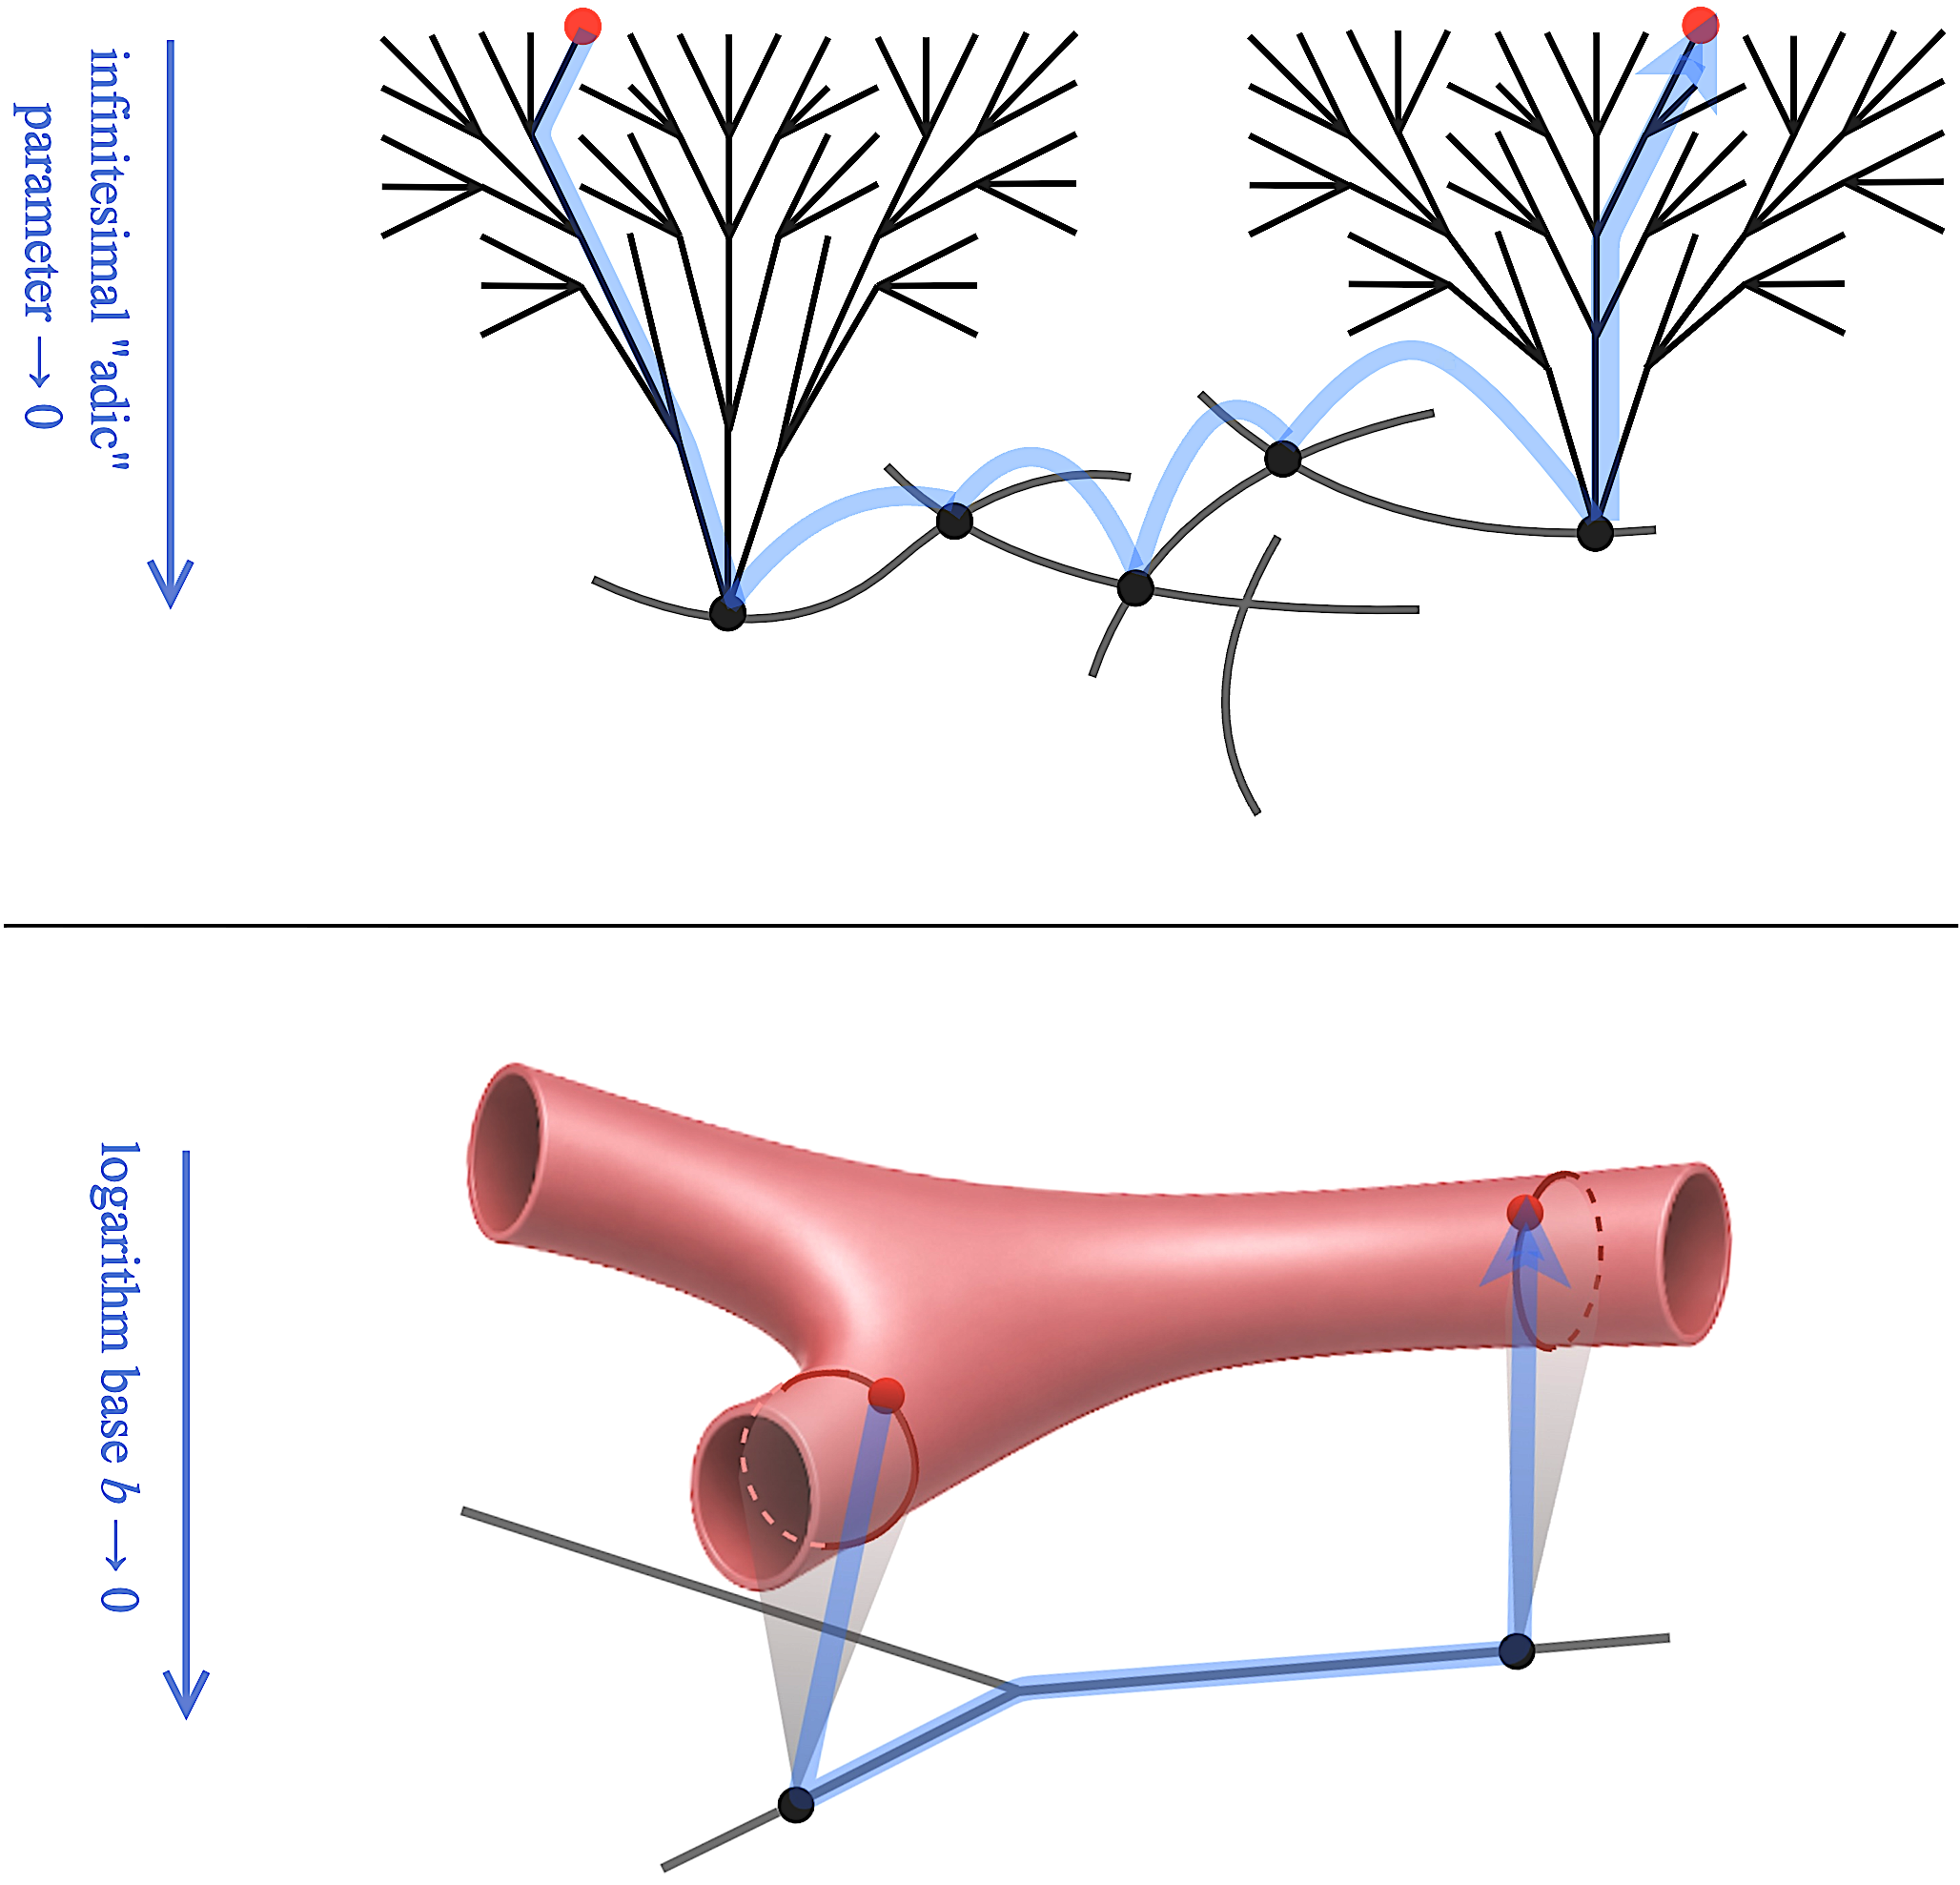
\includegraphics[scale=.25]{../../../assets/images/mathematical_model/log_contractions.png}
    $$
    \vskip -.2cm
    \caption{(Top) Non-Archimedean analytic, or ``{\em adic}'' geometry in as a curve collapses into a logarithmic pole. (Bottom) The degeneration of an amoeba down to a combinatorial curve as the base of its defining logarithm approaches $0$.}
    \label{fig: hierarchical paths}
\end{figure}


\end{document}
